\documentclass[12pt,conference]{IEEEtran}
\usepackage{tabularx} % in the preamble
\usepackage{hyperref}
\IEEEoverridecommandlockouts
\usepackage{xcolor}
\usepackage{nameref}
\usepackage{algorithm}
\usepackage{subfig}
\usepackage{dirtytalk}

\usepackage{fancyvrb}

\usepackage[noend]{algpseudocode}
\newcommand{\squeezeup}{\vspace{-2.5mm}}
% The preceding line is only needed to identify funding in the first footnote. If that is unneeded, please comment it out.
\usepackage{cite}
\usepackage[font={small}]{caption}
\usepackage{amsmath,amssymb,amsfonts}
\usepackage{graphicx}
\graphicspath{ {./images/} }
\usepackage{textcomp}
\usepackage{xcolor}
\def\BibTeX{{\rm B\kern-.05em{\sc i\kern-.025em b}\kern-.08em
    T\kern-.1667em\lower.7ex\hbox{E}\kern-.125emX}}
\begin{document}
\onecolumn
\title{ Predicting Underlying Heart Disease Using Binary Classification with Logistic Regression }
\author{\IEEEauthorblockN{Tyrone Lagore}
\IEEEauthorblockA{\textit{MADS} \\
\textit{University of Victoria}\\
Victoria, Canada \\
tyronelagore@uvic.ca \\V00995698}
}
\maketitle
\thispagestyle{plain}
\pagestyle{plain}
% \setlength{\parskip}{0.1cm plus4mm minus3mm}
\begin{abstract}
The WHO states that the leading cause of death globally is cardiovascular disease \cite{who}. It is important to diagnose heart disease early on, as management of the condition often includes life changes and medications that work as preventative measures. If a patient does not address the condition in time, it may lead to heart attack or other cardiovascular complications that require immediate medical intervention, and also have high mortality rates. Using a dataset acquired through \texit{Kaggle} that supplies various patient information and an identifier specifying weather or not the patient has underlying heart disease \cite{kaggle}, optimization techniques will be used to train a binary classification machine learning model on the data such that the model can be used to predict whether new unseen patients may have underlying heart disease. Various gradient descent methods will be compared to attempt to find an optimal model for this particular problem.
\end{abstract}

\section{Introduction}
\subsection{Heart Disease}
Heart disease is one of the leading causes of death worldwide. Having an estimated 17.9 million people having died in 2019, heart disease related deaths represents 32\% of all deaths worldwide \cite{who}. It is also a condition that is much better addressed through prevention. Should the disease progress to the point that a patient must seek medical attention, then it will be much more serious than if the patient had the condition diagnosed earlier on. 

Given a dataset obtained on Kaggle \cite{kaggle}, with various patient descriptors, several machine learning models will be trained in an attempt to create a binary classifier that can predict whether or not new unseen patients are at risk for having heart disease. Several gradient descent methods and one Newton method will be compared against one another to gauge the performance and select the best model.

\section{Data}
\subsection{Understanding the Features}
The dataset 918 samples, each sample has 11 features with 1 label depicting whether or not the patient has heart disease. The sample features are labeled as $X$ and assigned as $\begin{bmatrix}x_1, x_2, ... x_{918}\end{bmatrix} \in \mathbb{R}^{11\times 918}$, the label is assigned as $y \in \mathbb{R}^{918x1}$.

The 11 features and label can be described as seen in table \ref{tab:features}. Sex, ChestPainType, RestingECG, ExerciseAngina, and ST\_Slope are all categorical features and will need to be converted to numerical values before proceeding with training the models. 
 
\begin{table*}[t]
\centering
\caption{\label{tab:features}Dataset Features and Label\cite{kaggle} }
\begin{tabular}{||>{\centering}m{0.13\textwidth}>{\centering\arraybackslash}m{0.25\textwidth}>{\centering\arraybackslash}m{0.40\textwidth}||}
\hline
 Features & Description & Values\\ [0.5ex] 
\hline\hline
\vspace{.1cm}Age\vspace{.1cm} & Age of the patient in years 
                        & \vspace{.1cm}$x\in \mathbb{Z}$\vspace{.1cm}\\
\hline
\vspace{.1cm}Sex \vspace{.1cm} & Sex of the patient
                &\vspace{.1cm}[M]: Male, [F]: Female\vspace{.1cm}\\
\hline
\vspace{.1cm}ChestPainType \vspace{.1cm} & Resting blood pressure
                &\vspace{.1cm}[TA]: Typical Angina, [ATA]: Atypical Angina, [NAP]: Non-Anginal Pain, [ASY]: Asymptomatic\vspace{.1cm}\\
\hline
\vspace{.1cm}RestingBP \vspace{.1cm} & Chest pain type
                &\vspace{.1cm}$x\in \mathbb{R}$ [mm Hg]\vspace{.1cm}\\
\hline
\vspace{.1cm}Cholesterol \vspace{.1cm} & Serum cholesterol
                &\vspace{.1cm}$x\in \mathbb{Z}$ [mm/dl]\vspace{.1cm}\\
\hline
\vspace{.1cm}FastingBS \vspace{.1cm} & Fasting blood sugar
                &\vspace{.1cm}[1]: if FastingBS $>$ 120 mg/dl, [0]: otherwise\vspace{.1cm}\\
\hline
\vspace{.1cm}RestingECG \vspace{.1cm} & Resting electrocardiogram results
                &\vspace{.1cm}[Normal]: Normal, [ST]: having ST-T wave abnormality (T wave inversions and/or ST elevation or depression of $>$ 0.05 mV), [LVH]: showing probable or definite left ventricular hypertrophy by Estes' criteria]\vspace{.1cm}\\
\hline
\vspace{.1cm}MaxHR \vspace{.1cm} & Maximum heart rate achieved
                &\vspace{.1cm}$x \in \mathbb{Z}$\vspace{.1cm}\\
\hline
\vspace{.1cm}ExerciseAngina \vspace{.1cm} & Exercise-induced angina
                &\vspace{.1cm}[Y]: Yes, [N]: No\vspace{.1cm}\\
\hline
\vspace{.1cm}Oldpeak \vspace{.1cm} & ST depression induced by exercise relative to rest
                &\vspace{.1cm}$x \in \mathbb{R}$\vspace{.1cm}\\
\hline
\vspace{.1cm}ST\_Slope \vspace{.1cm} & The slope of the peak exercise ST segment
                &\vspace{.1cm}[Up]: upsloping, [Flat]: flat, [Down]: downsloping]\vspace{.1cm}\\
\hline
\vspace{.1cm}HeartDisease \vspace{.1cm} & Output class 
                &\vspace{.1cm}[1]: heart disease, [0]: Normal\vspace{.1cm}\\
\hline
\end{tabular}
\caption{\label{tab:numerical-features}Numerical Feature Information }
    \centering
    \begin{tabular}{|l|l|l|l|l|l|l|l|}
    \hline
        ~ & Age & RestingBP & Cholesterol & FastingBS & MaxHR & Oldpeak & HeartDisease \\ \hline
        count & 918 & 918 & 918 & 918 & 918 & 918 & 918 \\ \hline
        mean & 53.510893 & 132.396514 & 198.799564 & 0.233115 & 136.809368 & 0.887364 & 0.553377 \\ \hline
        std & 9.432617 & 18.514154 & 109.384145 & 0.423046 & 25.460334 & 1.06657 & 0.497414 \\ \hline
        min & 28 & 0 & 0 & 0 & 60 & -2.6 & 0 \\ \hline
        25\% & 47 & 120 & 173.25 & 0 & 120 & 0 & 0 \\ \hline
        50\% & 54 & 130 & 223 & 0 & 138 & 0.6 & 1 \\ \hline
        75\% & 60 & 140 & 267 & 0 & 156 & 1.5 & 1 \\ \hline
        max & 77 & 200 & 603 & 1 & 202 & 6.2 & 1 \\ \hline
    \end{tabular}
\end{table*}

It can be seen in table \ref{tab:numerical-features} that the values for the numerical features vary quite substantially. Some, such as FastingBS is between 0 and 1, whereas Cholesterol goes form 0 to 603. Furthermore, the presence of 0 in a field like RestingBP and Cholesterol most likely indicates that some of the samples are missing this feature information. It will be desirable to ensure that the features are scaled to be more in line with one another in order to ensure that the model can be trained effectively. This will be discussed more in section \ref{CleaningData}.

\subsection{Visualizing the Data}
Several of the fields are categorical, which must be translated to a numerical value before training the model. However, depending on the cleanliness of the dataset, some of the categories may have needlessly many categories. This could cause some categorical features to have samples that have a very small number of a certain type of category.

It is important to visualize the categorical fields to see if there are any categories that are vastly underrepresented. If they appear in small enough quantities, it may be acceptable to remove the samples from the dataset. The visualization of the categorical features can be seen in fig. \ref{fig:categories}. It does not seem that any of the categories have needlessly few representations in the samples, so it should be acceptable to keep every category of every categorical feature.

\begin{figure*}[t]
\centering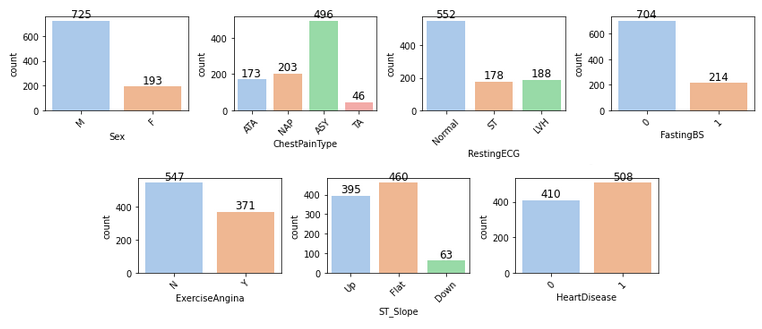
\includegraphics[width=\textwidth]{categories}
\caption{\label{fig:categories}Visualization of Categorical Features}
\end{figure*}

\subsection{Cleaning the Data}
\label{CleaningData}
\subsubsection{Categorical Features} 
To handle the categorical features, they must be converted to be numerical. One such method we can achieve this is through "One-Hot Encoding" the categories. We can transform one categorical feature into $n$ different features, one for each of the unique features in that category. Each new feature will be "one-hot" if the sample belonged to that category. For example, if a categorical feature $C^1$ had unique categories $\{c_1, c_2, ..., c_n\} \in C^1$, then we would add $n$ new features $\{C^1_{c1} C^1_{c2}, ..., C^1_{cn}\}$ and an individual sample that had category $c_i$ would then have the values for these features as
$$\begin{bmatrix}C^1_{c1}\\...\\C^1_{ci}\\...\\C^1_{cn}\end{bmatrix}^T = \begin{bmatrix}0\\...\\1\\...\\0\end{bmatrix}^T $$

As such, ChestPainType will be converted to a $1\times 4$ one-hot encoded feature, Sex $\in 1\times 2$, RestingECG $\in 1\times 3$, ExerciseAngina $\in 1\times 2$, ST\_Slope $\in 1\times 3$. The one-hot encoding transformed the dataset from 11 features with a mix of categorical and numerical features into 20 numerical features.

We can visualize the correlation between features through a heatmap as seen in fig \ref{fig:one-hot-heatmap}

\begin{figure}%
    \centering
    \subfloat[\centering Correlation before One-Hot Encoding]{{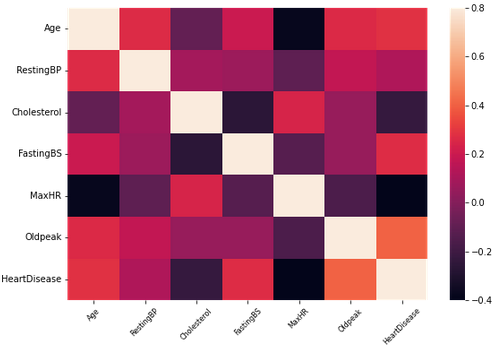
\includegraphics[width=.45\textwidth]{heatmap} }}%
    \qquad
    \subfloat[\centering Correlation after One-Hot Encoding]{{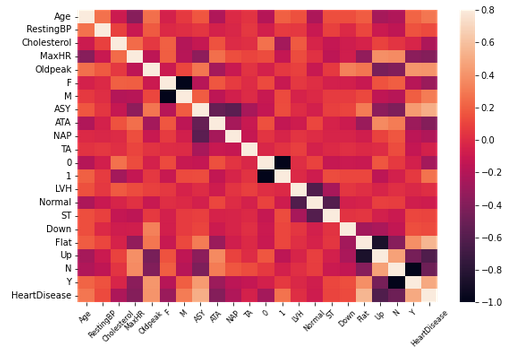
\includegraphics[width=.45\textwidth]{one-hot-heatmap} }}%
    \caption{Feature correlation viewed as heatmap}%
    \label{fig:one-hot-heatmap}%
\end{figure}

\subsubsection{Numerical Features}
There were two numerical features that were missing data, Cholesterol and RestingBP. Since there was only one sample missing the RestingBP information, this sample was simply dropped from the dataset. Cholesterol, however, was missing quite a few samples. It was decided to simply replace the missing cholesterol features with the mean of the existing cholesterol data, as grouped by male and female. 

Instead of just using the mean, a thought was to build a linear regression model that would use the other numerical features to predict the cholesterol level. However, since cholesterol level had a poor correlation with heart disease, more effort was not invested in removing the bias from this decision and the missing values were simply replaced with the mean for male and female respectively.

\subsubsection{Splitting test and Training Data}
The dataset was then split into training and testing data. 20\% of the data was set aside as test data and the remaining 80\% for testing. The sklearn function \verb|train_test_split| was used to separate the test and training data, stratified on the feature labels (HeartDisease) \cite{sklearn}. 

\vspace{0.3cm}
\begin{minipage}{0.89\linewidth}
\begin{Verbatim}[numbers=left,framesep=3mm]
train_test_split(X, y, 
    test_size=0.20, 
    random_state=int(time.time()), 
    stratify=y)
\end{Verbatim}
\end{minipage}
\vspace{0.5cm}

\subsubsection{Scaling the Features}
Since the numerical features are in quite a different range from one another, especially with the addition of many one-hot columns, it is important to scale the features to be within a reasonable range of one another. Therefore the decision was to normalize each numerical column (but not the one-hot columns) using z-score normalization. That is, the values of each $x_p$ in the feature $i$ were replaced with the following formulation:

$$ Z_p = \frac{x_p - \mu_i}{\sigma_i} $$

Where $\mu_i$ is the mean, and $\sigma_i$ is the standard deviation of feature $i$. $\mu$ and $\sigma$ were calculated on the training data, then simply applied to the test data using the same $\mu$ and $\sigma$. This is because we will not know the true mean and standard deviation of new data, so we assume that it falls in line with our current knowledge based on the data that we train on.

Using sklearn's StandardScaler class, we can achieve the above scaling:

\vspace{0.3cm}
\begin{minipage}{0.89\linewidth}
\begin{Verbatim}[numbers=left,framesep=3mm]
from sklearn.preprocessing 
        import StandardScaler
scaler = StandardScaler()
scaler.fit(
    X_train[columns_to_scale])

X_train[columns_to_scale] = 
    scaler.transform(
        X_train[columns_to_scale])
        
X_test[columns_to_scale] = 
    scaler.transform(
        X_test[columns_to_scale])
\end{Verbatim}
\end{minipage}
\vspace{0.5cm}

\section{Training the Models}
\subsection {Binary Classification}
The desired output of the model is a simple confirmation of "yes", this sample is at risk for having underlying heart disease, or "no" the sample is not at risk for having underlying heart disease. The task of determining if a sample belongs to one of two classes is a classic binary classification problem. As such, logistic regression will be used to train the models.
\subsubsection {Loss Function}
The logistic regression loss function is defined as
$$\frac{1}{P}\sum_{p=1}^{P} \log\left(\frac{1}{1+e^{-y_p(\^w^Tx_p)}}\right) $$

Intuitively, we are trying to define a probability that this sample belongs to the class, where $y = 1$ when the sample belongs to this class and $y = -1$ when the sample does not belong to this class. The logistic regression loss function will heavily penalize when the sample is far away from our desired value.

A regularization term can be added to the loss function in order to amplify the error of our function.

$$ \frac{1}{P}\sum_{p=1}^{P} \log\left(\frac{1}{1+e^{-y_p(\^w^Tx_p)}}\right) + \frac{\mu}{2}||\^w||_2^2$$

This will cause the model to perform more poorly on training data, but by preventing over-fitting on the training data - the regularization aims to perform better on unseen samples. 


\subsection {Gradient Descent}
The general form of optimization algorithms can be seen in algorithm \ref{alg:optimization}.
\begin{algorithm}
\caption{Generic Optimization Algorithm \cite{course-notes}}
\label{alg:optimization}
\begin{algorithmic}[1]
\State Algorithm parameters: initial point $x_0$
\State convergence tolerance $\epsilon$, $k = 0$
\While {not converged}
    \State Given $x_k$ find search direction $d_k$ by appropriate procedure
    \State Compute $\alpha_k > 0$ that minimizes $f(x_k + \alpha_kd_k)$
    \State $x_{k+1} = x_k + \alpha_kd_k$
    \If{$||\alpha_k d_k|| < \epsilon$}
        \State Output $x_k$
    \EndIf
    \State $k = k+1$
\EndWhile 
\end{algorithmic}
\end{algorithm}

For generic gradient descent, $d_0$ is calculated as $-\nabla f(x_k)$ and $\alpha_k$ is calculated using backtracking line search, as seen in algorithm \ref{alg:line-search}

\begin{algorithm}
\caption{Backtracking Line Search \cite{course-notes}}
\label{alg:line-search}
\begin{algorithmic}[1]
\State Algorithm parameters: initial point $x_k$
\State Descent direction $d_k$ at $x_k$
\State Select constants $\rho \in (0, 0.5)$ and $\gamma \in (0,1)$
\State Set $\alpha=1$
\While {$f(x_k + \alpha d_k) > f(x_k) + \rho \alpha g_k^T d_k $}
    \State $\alpha = \gamma \alpha$
\EndWhile 
\State Output $\alpha_k = \alpha$
\end{algorithmic}
\end{algorithm}

However, generic gradient descent methods are inherently slow for most functions. This is due to the fact that any two search directions that are successively calculated will be orthogonal to one another. This creates a zig-zag of search directions that is only ever efficient if the condition number of the Hessian of the function is low, that is: the contour of the function is not steep. \cite{course-notes}. Practically speaking, this is rarely the case. As a result, there are many optimized algorithms that can help us to achieve superior performance.

\subsection {Conjugate Gradient Descent (CG)}
Intuitively, Conjugate Gradient Descent methods attempt to take some information from the previously calculated descent direction. Since they are orthogonal to one another, then some combination of the two descent directions points towards the actual minimizer of the function. As such, the descent direction is calculated slightly differently by first extracting some information about the relation of the consecutive gradients \cite{course-notes}:

$$\beta_k^{PRP} = \frac{\nabla f(x_k)^T \gamma_{k-1}}{||\nabla f(x_{k-1})||^2_2} $$ where
$$\gamma_{k-1} = \nabla f(x_k) - \nabla f(x_{k-1})$$

Finally, the descent direction can be calculated using $d_k = -\nabla f(x_k) + \beta_kd_{k-1}$. The accuracy and time to calculate using this algorithm can be seen in table \ref{tab:results}.

\subsection {Newton Algorithm}
The Newton algorithm attempts to improve the descent direction by including the quadratic estimation as part of the descent direction. In many scenarios, this can become infeasible due to the size of the dataset, as the Newton algorithm involves calculating the inverse of the Hessian. Considering that the heart disease dataset is small, it is feasible to use the newton algorithm to train our classifier. With the Newton algorithm, the descent direction is calculated as:

$$d_k = -\nabla^2f(x_k)^{-1}\nabla f(x_k)$$

$\alpha$ in the case of the Newton algorithm is always equal to 1, and therefore does not need to be computed using the backtracking line search. The accuracy and time to calculate using this algorithm can be seen in table \ref{tab:results}.

\subsection {Broyden-Fletcher-Goldfarb-Shanno (BFGS)}
The Newton algorithm is not always feasible due to the intensive computation required when performing the inverse of the Hessian. As such, methods have arisen that allow the \textit{approximation} of the Hessian inverse. This is done using only gradient information, iteratively updating some matrix $S_k$ such that it approximates the Hessian inverse. As such, the update direction is the same as the Newton algorithm, replacing the Hessian inverse with

$$ d_k = -S_k \nabla f(x_k) $$

Initially, $S_k$ is set to the identity matrix. Initially, compute:
$$ \delta_k = x_{k+1} - x_{k}, \gamma = \nabla f(x_{k+1}) - \nabla f(x_k) $$

Then with each iteration, $S_{k+1}$ is calculated as:
$$ S_k + \left( 1 + \frac{\gamma_k^T S_k \gamma_k}{\gamma_k^T \delta_k} \right) \frac{\delta_k \delta_k^T}{\gamma_k^T\delta_k} - \frac{\delta_k \gamma_k^T S_k + S_k \gamma_k \delta_k^T}{\gamma_k^T\delta_k} $$

See table \ref{tab:results} for the accuracy and time to calculate using the BFGS algorithm.
\subsection {Memoryless BFGS}
Although the BFGS algorithm is excellent for mitigating the computational overhead that the Newton method incurs through the Hessian inverse calculation, it still has a downside. That is, the size of $S_k$ can become increasingly large over time, which can become infeasible to hold in memory on large datasets. the Memoryless BFGS algorithm rewrites the above update rule to compute several inner products.

$$ \rho = \frac{1}{\gamma^T_k \delta_k}, t_k = \delta_k^T \nabla f(x_k+1),$$
$$and\ q_k = \nabla f(x_{k+1}) - \rho_kt_k\gamma_k$$

Then the search direction is calculated as

$$ d_{k+1} = \rho_k (\gamma_k^T q_k - t_k ) \delta_k - q_k $$

The heart disease dataset is quite small, so the memory savings provided by this algorithm is inconsequential for this dataset. However, to see how it performs on this data, the model was trained and the results can be seen in table \ref{tab:results}

\section{Results}
\label{Results}
\begin{table}[!ht]
\caption{\label{tab:results}Best Results }
    \centering
    \begin{tabular}{|l|>{\centering}l|>{\centering}l|>{\centering}l|>{\centering}l|>{\centering}l l|}
    \hline
        ~ & Time (s) & Accy (\%) & $\mu$ & Iters & C. & Matrix \\ \hline
        BFGS & 0.0112 & 76.0870 & 0 & 9 & 95 & 37 \\
        ~ & ~ & ~ & ~ & ~ & 7 & 45 \\ \hline
        ML-BFGS & 0.6191 & 84.7826 & 0.1 & 263 & 89 & 15 \\
        ~ & ~ & ~ & ~ & ~ & 13 & 67 \\ \hline
        CG & 0.2557 & 84.2391 & 0.1 & 152 & 89 & 16 \\
        ~ & ~ & ~ & ~ & ~ & 13 & 66 \\ \hline
        Newton & 0.0048 & 86.4130 & 0 & 1 & 90 & 13 \\ \
        ~ & ~ & ~ & ~ & ~ & 12 & 69 \\ \hline
    \end{tabular}
\end{table}

Several iterations were run with different values for $mu$ and table \ref{tab:results} were the $mu$ that had the best accuracy.
Furthermore, the data was cleaned in various ways including:
\begin{itemize}
    \item \textbf{A}: Not normalizing the data
    \item \textbf{B}: Removing the Cholesterol feature instead of filling it missing values with mean
    \item \textbf{C}: Removing the 0 valued Cholesterol samples instead of filling missing values with mean
    \item \textbf{D}: Filling the missing Cholesterol values with mean and normalizing the dataset using z-score normalization
\end{itemize}

Dataset \textbf{D} performed better than any of the other methods of cleaning, table \ref{tab:results} represents the results run on this dataset. When normalization was not used, most algorithms took a lot longer to converge, and sometimes with worse results. As seen in table \ref{tab:bad-results}, CG took 9106 iterations to converge, taking a total of 64 seconds to exactly the same accuracy as with the normalized dataset. Newton performed admirably, achieving the same accuracy in only slightly longer time. ML-BFGS was the only algorithm that saw a slight increase to its accuracy, with a moderate hit to the computation time. BFGS struggled greatly, at 55.4348\% accuracy, and came to a solution that could almost be obtained by randomly guessing.

\begin{table}[!ht]
\caption{\label{tab:bad-results}Non-Scaled Results }
    \centering
    \begin{tabular}{|l|l|l|l|l|}
    \hline
        ~ & Time (s) & Accy ($\backslash$\%) & Mu & Iterations \\ \hline
        BFGS & 0.0324 & 55.4348 & 0 & 14 \\ \hline
        ML-BFGS & 2.3007 & 85.3261 & 0.1 & 610 \\ \hline
        CG & 64.3264 & 84.2391 & 0.1 & 9106 \\ \hline
        Newon & 0.0308 & 86.4130 & 0 & 1 \\ \hline
    \end{tabular}
\end{table}

Overall, the Newton algorithm was the most effective in terms of accuracy and time taken to calculate. However, this is most likely to do with the size of the dataset allowing for a quick inverse calculation - in addition to the fact that Newton only needed to run for 1 iteration to achieve it's optimal parameters. ML-BFGS and CG methods performed similarly on the dataset, with CG having a slightly faster computation and slightly lower accuracy. Surprisingly, BFGS performed vastly worse than all of the other algorithms.

\section{Discussion}
Due to the results of the classifiers seen in \nameref{Results}, it seems that there may have been some limiting factors in this dataset that prevented more accurate results. This may have been due to the data not having features that can help to accurately predict heart disease, or more likely the cause is in the preparation of the data for testing. As the data had many different categorical variables, different labeling methods may have produced superior results. The use of one-hot features for every categorical feature created a sparse dataset, that may not have been as ideal in calculating better accuracy parameters. Some additional domain knowledge into what each category represents might give better methods to label them. For example, if ChestPainType represents some type of scale of chest pain that gradually increases, using a label for each category that scales with the chest pain type (1, 2, 3, ...) might have produced superior results. The dataset was also not as large as might be hoped. Having more samples to draw upon, in addition to other features, might produce more effective models. However, at 86.4\% accuracy, the newton model still offers a reasonably accurate classifier.

In terms of the most effective predictor, Newton not only had the best accuracy - but also had the fewest false negatives. This would be very important in terms of creating a classifier that might be used for recommending patients be tested for heart disease or not. Should the model tell them they do not have concern for underlying heart disease, and they \textbf{do} have underlying heart disease, it would be much worse than telling someone they have heart disease when they do not.

\section{Conclusion}
It was interesting to see how the finding of quality data that also had an acceptable quantity was the most difficult part about creating the classifier. The way in which the data is pre-processed vastly changes the quality of the resultant models. While the data was not as high-quality as would have been desired, it is rarely the case that the data conforms exactly to how we would like it to be. As data processing is an essential part of the process, a lot was learned in how to properly prepare the data such that it produces effective models.

The entirety of the code for this project, and the data, can be found in this github repository: \href{https://github.com/tlagore/ece503\_final\_project}{https://github.com/tlagore/ece503\_final\_project}

\begin{thebibliography}{00}
\bibitem{who} World Health Organization, “Cardiovascular Diseases (CVDs),” who.int, 2021. https://www.who.int/news-room/fact-sheets/detail/cardiovascular-diseases-(cvds).
\bibitem{kaggle} “Heart Failure Prediction Dataset,” kaggle.com. https://www.kaggle.com/fedesoriano/heart-failure-prediction.
\bibitem{sklearn} F. Pedregosa et al., “Scikit-learn: Machine learning in Python”, Journal of machine learning research, vol 12, no Oct, bll 2825–2830, 2011.
\bibitem{course-notes}Lu, Wu-Sheng “Optimization for Machine Learning” ECE 403/503 Course Notes - https://studentweb.uvic.ca/~leizhao/403-2021/Notes403-503-2021.pdf
\end{thebibliography}

\onecolumn

\begin{appendices}
\appendix
\subsection{Matlab Code}
\subsubsection{Main Driver}
\label{AppendixA-Main}
\begin{verbatim}
[Xtr, y_tr, Xte, y_te] = 
    lr_train_and_predict('heart_cleaned_filled_scaled.csv');

function [Xtr, y_tr, Xte, y_te] =  lr_train_and_predict(file_name)
    [Xtr, y_tr, Xte, y_te, num_features] = 
        load_and_prepare_lr_data(file_name);

    tic
    mu = 0.01;
    w0 = zeros(num_features+1, 1);
    [xs, ~, ~] = bfgs_ML('f_elw', 'g_elw', w0, 1e-9, [Xtr; y_tr], mu);
    disp("Trained ws_1 with confusion matrix")
    disp("Confusion against test data:")
    [confusion, accuracy] = evaluate_lrbc(Xte, y_te, xs);
    disp(confusion);
    fprintf("bfgs_ML, mu=%f: Accuracy of %%%.6f on test data\n\n", 
        mu, accuracy)
    disp(toc)
    
    tic
    w0 = zeros(num_features+1, 1);
    [xs, ~, ~] = bfgs('f_elw', 'g_elw', w0, 1e-9, [Xtr; y_tr], mu);
    disp("Trained ws_1 with confusion matrix")
    disp("Confusion against test data:")
    [confusion, accuracy] = evaluate_lrbc(Xte, y_te, xs);
    disp(confusion);
    fprintf("bfgs, mu=%f: Accuracy of %%%.6f on test data\n\n", mu, accuracy)
    disp(toc)
    
    tic
    mu = 0.1;
    w0 = zeros(num_features+1, 1);
    [xs, ~, ~] = cg('f_elw', 'g_elw', w0, 1e-9, [Xtr; y_tr], mu);
    disp("Trained ws_1 with confusion matrix")

    disp("Confusion against test data:")
    [confusion, accuracy] = evaluate_lrbc(Xte, y_te, xs);
    disp(confusion);
    fprintf("cg, mu=%f: Accuracy of %%%.6f on test data\n\n", mu, accuracy)
    disp(toc)

    tic
    mu = 0.1;
    [xs, confusion] = LRBC_newton(Xtr, y_tr, 1);
    disp("Trained ws_1 with confusion matrix")
    disp(confusion)

    disp("Confusion against test data:")
    [confusion, accuracy] = evaluate_lrbc(Xte, y_te, xs);
    disp(confusion);
    fprintf("newton, iterations=1: Accuracy of %%%.6f on test data\n\n", 
        mu, accuracy)
    disp(toc)
end

function [Xtr, y_tr, Xte, y_te, num_features] = 
        load_and_prepare_lr_data(file_name)
    X = readmatrix(file_name);

    [num_rows, total_samples] = size(X);
    num_features = num_rows - 1;

    train_size = floor(total_samples*0.8);

    Xtr = X(1:num_features,1:train_size);
    y_tr = X(num_features+1,1:train_size);

    Xte = X(1:num_features,train_size+1:total_samples);
    y_te = X(num_features+1,train_size+1:total_samples);

    % conform our labels to logistic regression
    % -1 instead of 0
    y_tr(y_tr == 0) = -1;
    y_te(y_te == 0) = -1;
end
\end{verbatim}

\subsection{Algorithms}
\subsubsection{Conjugate Gradient Descent}
\label{AppendixB-CG}
\begin{verbatim}
% To implement CG algorithm with Polak-Ribiere-Polyak-(plus)'s beta.
% Example:
% [xs,fs,k] = cg('f_rosen','g_rosen',[-1;-1],1e-6);
function [xs,fs,k] = cg(fname,gname,x0,epsi,D,mu)
format compact
format long
n = length(x0);
k = 0;
xk = x0;
gk = feval(gname,xk,D,mu);
dk = -gk;
er = norm(gk);
while er >= epsi
    ak = bt_lsearch2019(xk,dk,fname,gname,D,mu);
    xk_new = xk + ak*dk;  
    gk_new = feval(gname,xk_new,D,mu);
    gmk = gk_new - gk;
    bk = max((gk_new'*gmk)/(gk'*gk),0);
    dk = -gk_new + bk*dk;
    xk = xk_new;
    gk = gk_new;
    er = norm(gk);
    k = k + 1;
end
% disp('solution:')
xs = xk;
disp('objective function at solution point:')
fs = feval(fname,xs,D,mu);
format short
disp('number of iterations at convergence:')
k
\end{verbatim}

\subsubsection{Newton Algorithm}
All algorithms were taken from the course website and modified slighty to make use of 
\label{AppendixB-Newton}
\begin{verbatim}
% Logistic regression for binary classification using Newton algorithm.
% Inputs:
% X: input data matrix where input samples are given as colum vectors.
% y: a vector whose pth component is the label for the pth input sample,
%    which is set to 1 if the pth sample belongs to class P, or set to
%    -1 if the pth sample belongs to class N.
% K: number of Newton iterations.
% Outputs:
% ws: a column vector of optimized weight w* and bias b*.
% C2: 2 x 2 confusion matrix.
% Written by W.-S. Lu, University of Victoria.
% Last modified: May 16, 2020.
% Example: 
% Dp = [1.5 3.5 5 6.9 8.4 10 11.2; 6.5 6.5 5 3.7 2.6 5 1.5];
% Dn = [1 2.1 3.1 4 5.9 7.9 9 10.5; 4.5 3.5 4.9 4.2 2.7 2.2 1.6 0.8];
% X = [Dp Dn];
% y = [ones(1,7) -ones(1,8)];
% [ws,C2] = LRBC_newton(X,y,5);
function [ws,C2] = LRBC_newton(X,y,K)
y = y(:)';
[N,P] = size(X);
N1 = N + 1;
Ine = 1e-10*eye(N1);
ind = 1:1:P;
indp = find(y > 0);
indn = setdiff(ind,indp);
Xh = [X; ones(1,P)];
Xp = Xh(:,indp);
Xn = Xh(:,indn);
Xw = [Xp -Xn];
P1 = length(indp);
k = 0;
wk = zeros(N1,1);
while k < K
  gk = feval('g_LRBC',wk,Xw);
  Hk = feval('h_LRBC',wk,Xw) + Ine;
  dk = -Hk\gk;
  ak = bt_lsearch2019(wk,dk,'f_LRBC','g_LRBC',Xw);
  wk = wk + ak*dk;
  k = k + 1;
end
ws = wk;
yt = sign(ws'*[Xp Xn]);
er = abs(y-yt)/2;
erp = sum(er(1:P1));
ern = sum(er(P1+1:P));
C2 = [P1-erp ern; erp P-P1-ern];
\end{verbatim}

\subsubsection{BFGS}
\label{AppendixB-BFGS}
\begin{verbatim}
% To implement BFGS algorithm.
% Example:
% [xs,fs,k] = bfgs('f200','g200',[zeros(100,1);-ones(100,1)],1e-7);
function [xs,fs,k] = bfgs(fname,gname,x0,epsi,D,mu)
format compact
format long
n = length(x0);
I = eye(n);
k = 1;
xk = x0;
Sk = I;
fk = feval(fname,xk,D,mu);
gk = feval(gname,xk,D,mu);
dk = -Sk*gk;
ak = bt_lsearch2019(xk,dk,fname,gname,D,mu);
dtk = ak*dk;
xk_new = xk + dtk;
fk_new = feval(fname,xk_new,D,mu);
dfk = abs(fk - fk_new);
er = max(dfk,norm(dtk));
while er >= epsi
      gk_new = feval(gname,xk_new,D,mu);
      gmk = gk_new - gk;
      D = dtk'*gmk;
      if D <= 0
         Sk = I;
      else
         sg = Sk*gmk;
         sw0 = (1+(gmk'*sg)/D)/D;
         sw1 = dtk*dtk';
         sw2 = sg*dtk';
         Sk = Sk + sw0*sw1 - (sw2'+sw2)/D;
      end
      fk = fk_new;
      gk = gk_new;
      xk = xk_new;
      dk = -Sk*gk;
      ak = bt_lsearch2019(xk,dk,fname,gname,D,mu);
      dtk = ak*dk;
      xk_new = xk + dtk;
      fk_new = feval(fname,xk_new,D,mu);
      dfk = abs(fk - fk_new);
      er = max(dfk,norm(dtk));
      k = k + 1;
end
disp('solution:')
xs = xk_new
disp('objective function at solution point:')
fs = feval(fname,xs,D,mu)
format short
disp('number of iterations at convergence:')
k
\end{verbatim}

\subsubsection{ML-BFGS}
\label{AppendixB-MLBFGS}
\begin{verbatim}
% To implement memoryless BFGS algorithm
% Example: [xs,fs,k] = bfgs_ML('f_rosen','g_rosen',[0;2],1e-6);
function [xs,fs,k] = bfgs_ML(fname,gname,x0,epsi,D,mu)
format compact
format long
k = 1;
xk = x0;
fk = feval(fname,xk,D,mu);
gk = feval(gname,xk,D,mu);
dk = -gk;
ak = bt_lsearch2019(xk,dk,fname,gname,D,mu);
dtk = -ak*gk;
xk_new = xk + dtk;
fk_new = feval(fname,xk_new,D,mu);
dfk = abs(fk - fk_new);
er = max(dfk,norm(dtk));
while er >= epsi
      gk_new = feval(gname,xk_new,D,mu);
      gmk = gk_new - gk;
      gk = gk_new;
      rk = 1/(dtk'*gmk);
      if rk <= 0
         dk = -gk;
      else
         tk = dtk'*gk;
         qk = gk - (rk*tk)*gmk;
         bk = rk*(gmk'*qk - tk);
         dk = bk*dtk - qk;
      end
      fk = fk_new;
      xk = xk_new;
      ak = bt_lsearch2019(xk,dk,fname,gname,D,mu);
      dtk = ak*dk;
      xk_new = xk + dtk;
      fk_new = feval(fname,xk_new,D,mu);
      dfk = abs(fk - fk_new);
      er = max(dfk,norm(dtk));
      k = k + 1;
end
disp('solution:')
xs = xk_new
disp('objective function at solution point:')
fs = feval(fname,xs,D,mu)
format short
disp('number of iterations at convergence:')
k
\end{verbatim}

\subsubsection{Back-Tracking Line Search}
\label{AppendixB-BTLS}
\begin{verbatim}
%  Program: bt_lsearch2019.m
%  Implements line learch by backtracking.
%  Description: Implements inexact line search described in 
%  Reference: Sec. 9.2 of Boyd and Vanderberghe's book.
%  Input:
%     x:  initial point
%     d:  search direction
% fname:  objective function to be minimized along the direction of s  
% gname:  gradient of the objective function.
%    p1:  user-defined parameter vector whose components mast have been 
%         numerically specified. The order in which the components of p1 
%         appear must be the same as what they appear in fname and gname.
%         Note: p1 is an optional input.
%    p2:  2nd user-defined parameter vector whose components mast have been 
%         numerically specified. The order in which the components of p2 
%         appear must be the same as what they appear in fname and gname.
%         Note: p2 is an optional input.
% Output:
%     a:  acceptable value of alpha.
% Written by W.-S. Lu, University of Victoria.
% Last modified: July 28, 2019.
function a = bt_lsearch2019(x,d,fname,gname,p1,p2)
rho = 0.1;
gma = 0.5;
x = x(:);
d = d(:);
a = 1;
xw = x + a*d;
parameterstring ='';
if nargin == 5
   if ischar(p1)
      eval([p1 ';']);
   else
      parameterstring = ',p1';
   end
end
if nargin == 6
   if ischar(p1)
      eval([p1 ';']);
   else
      parameterstring = ',p1';
   end
   if ischar(p2)
      eval([p2 ';']);
   else
      parameterstring = ',p1,p2';
   end
end
eval(['f0 = ' fname '(x' parameterstring ');']);
eval(['g0 = ' gname '(x' parameterstring ');']);
eval(['f1 = ' fname '(xw' parameterstring ');']);
t0 = rho*(g0'*d);
f2 = f0 + a*t0;
er = f1 - f2;
while er > 0
     a = gma*a;
     xw = x + a*d;
     eval(['f1 = ' fname '(xw' parameterstring ');']);
     f2 = f0 + a*t0;
     er = f1 - f2;
end
if a < 1e-5
   a = min([1e-5, 0.1/norm(d)]); 
end 
\end{verbatim}
\end{appendices}
\end{document}